\documentclass[12pt,a4paper]{article}

% Báo cáo ưu tiên XeLaTeX/LuaLaTeX. Khối pdfTeX được giữ làm fallback.
\usepackage{iftex}
\ifPDFTeX
  \usepackage[T5]{fontenc}
  \usepackage[utf8]{inputenc}
  \usepackage{lmodern}
\else
  \usepackage{fontspec}
  \IfFontExistsTF{Times New Roman}
    {\setmainfont{Times New Roman}}
    {\setmainfont{TeX Gyre Termes}}
  \IfFontExistsTF{Consolas}
    {\setmonofont{Consolas}}
    {\setmonofont{DejaVu Sans Mono}}
\fi

\usepackage[english,vietnamese]{babel}
\usepackage{amsmath,amssymb}
\usepackage{booktabs,longtable,tabularx,array}
\usepackage{enumitem}
\usepackage[a4paper,margin=2.2cm,headheight=16pt]{geometry}
\usepackage{xcolor,graphicx}
\usepackage{microtype}
\usepackage{fancyhdr}
\usepackage{hyperref,bookmark}
\usepackage{caption,float}
\usepackage{listings}
\usepackage{tikz}
\usetikzlibrary{arrows.meta,positioning,shapes.geometric}

\definecolor{brandblue}{HTML}{164E78}
\definecolor{brandgreen}{HTML}{2E7D61}
\definecolor{softblue}{HTML}{EAF4FB}
\definecolor{softgray}{HTML}{F2F4F7}
\definecolor{warningorange}{HTML}{B85C00}
\definecolor{codegray}{HTML}{F7F7F7}

\hypersetup{
  colorlinks=true,
  linkcolor=brandblue,
  urlcolor=brandblue,
  citecolor=brandblue,
  pdftitle={WIP 4 tuần -- Tech Doc và Demo 3D Container Packing},
  pdfauthor={Dự án 3D Container Packing}
}

\pagestyle{fancy}
\fancyhf{}
\lhead{WIP 4 tuần -- 3D Container Packing}
\rhead{Tech Doc và Demo cơ bản}
\cfoot{\thepage}
\renewcommand{\headrulewidth}{0.4pt}
\setlength{\parindent}{0pt}
\setlength{\parskip}{0.55em}
\setcounter{tocdepth}{2}

\newcolumntype{Y}{>{\raggedright\arraybackslash}X}
\newcommand{\code}[1]{\texttt{\detokenize{#1}}}
\newcommand{\good}[1]{\textcolor{brandgreen}{\textbf{#1}}}
\newcommand{\warning}[1]{\textcolor{warningorange}{\textbf{#1}}}

\lstset{
  basicstyle=\ttfamily\small,
  backgroundcolor=\color{codegray},
  frame=single,
  rulecolor=\color{softgray},
  breaklines=true,
  columns=fullflexible,
  keepspaces=true,
  showstringspaces=false
}

% Hỗ trợ build từ project root hoặc từ docs/reports/explore.
\graphicspath{{../../assets/}{docs/assets/}}

\title{\textbf{WIP 4 tuần -- 3D Container Packing}\\[0.5em]
       \large Tech Doc và kịch bản demo cơ bản}
\author{Nhóm Mobility -- Freight}
\date{15 tháng 8 năm 2026}

\begin{document}

\begin{titlepage}
  \centering
  \vspace*{2.2cm}
  {\color{brandblue}\rule{\textwidth}{1.2pt}}\\[1.2cm]
  {\Huge\bfseries WIP 4 tuần\\[0.4em]3D Container Packing\par}
  \vspace{0.8cm}
  {\Large Tech Doc và kịch bản demo cơ bản\par}
  \vspace{1.2cm}
  {\large Service tối ưu xếp kiện vào kho container dị thể\par}
  \vfill
  \begin{tabular}{rl}
    \textbf{Phạm vi evidence:} & Level 1--5 \\
    \textbf{Trạng thái:} & WIP nghiên cứu đã qua validation phần mềm \\
    \textbf{Demo đề xuất:} & Streamlit Level 2, 15 phút \\
    \textbf{Ngày cập nhật:} & 15/08/2026
  \end{tabular}
  \vfill
  {\color{brandblue}\rule{\textwidth}{1.2pt}}
\end{titlepage}

\pagenumbering{roman}
\tableofcontents
\clearpage
\pagenumbering{arabic}

\section*{Tóm tắt dành cho PM}
\addcontentsline{toc}{section}{Tóm tắt dành cho PM}

Sản phẩm WIP là một service nghiên cứu giúp lựa chọn container và đề xuất vị trí xếp các
kiện hộp chữ nhật trong không gian 3D. Người dùng cung cấp danh sách kiện và kho container;
hệ thống trả về container được sử dụng, tọa độ, hướng đặt, chi phí thử nghiệm, mức sử dụng
sức chứa và mô hình 3D tương tác.

Sau bốn tuần, luồng chính từ dữ liệu đến nghiệm, kiểm định và hiển thị đã hoạt động. Phạm
vi đã có evidence gồm hình học, tải trọng, hỗ trợ hình học, xoay ngang, quy tắc chồng xếp
và truyền tải trọng tĩnh. Mọi nghiệm được báo thành công đều phải qua validator độc lập;
solver tự báo \code{FEASIBLE} chưa đủ để được công nhận.

\begin{center}
\fcolorbox{brandblue}{softblue}{\parbox{0.92\textwidth}{
\textbf{Thông điệp chính.} Đây là nền tảng R\&D đã nghiệm thu theo contract phần mềm
Level 1--5. Sản phẩm chưa phải hệ thống chứng nhận an toàn vận tải và chưa có production SLA.
}}
\end{center}

\section{Bài toán và giá trị hiện tại}

\subsection{Đầu vào}
\begin{itemize}[leftmargin=1.5em]
  \item Kích thước, khối lượng và định danh từng kiện.
  \item Kích thước, tải trọng, chi phí và số lượng physical container trong kho.
  \item Level ràng buộc, thuật toán, giới hạn container và thời gian tìm kiếm.
  \item Tùy chọn tìm kiếm toàn kho và cải thiện nghiệm sau construction.
\end{itemize}

\subsection{Đầu ra}
\begin{itemize}[leftmargin=1.5em]
  \item Danh sách container thực sự được dùng; vị trí và hướng đặt từng kiện.
  \item Số container, tổng chi phí, utilization và thời gian xử lý.
  \item Báo cáo kiểm định độc lập, diagnostics và lý do thất bại nếu không có nghiệm.
  \item Mô hình 3D có thể xoay, zoom và xem thông tin từng kiện.
\end{itemize}

\subsection{Giá trị đã chứng minh}
\begin{itemize}[leftmargin=1.5em]
  \item Loại sớm yêu cầu chắc chắn thiếu sức chứa theo thể tích hoặc tải trọng.
  \item Tìm tổ hợp trong toàn bộ kho physical container thay vì chỉ lấy một prefix cố định.
  \item So sánh nhiều constructor trên cùng input, constraint và deadline.
  \item Giữ nghiệm hợp lệ nếu repair hoặc bước cải thiện hết thời gian.
  \item Lưu manifest, checksum, config, seed và output theo từng run để tái lập.
\end{itemize}

\begin{figure}[H]
  \centering
  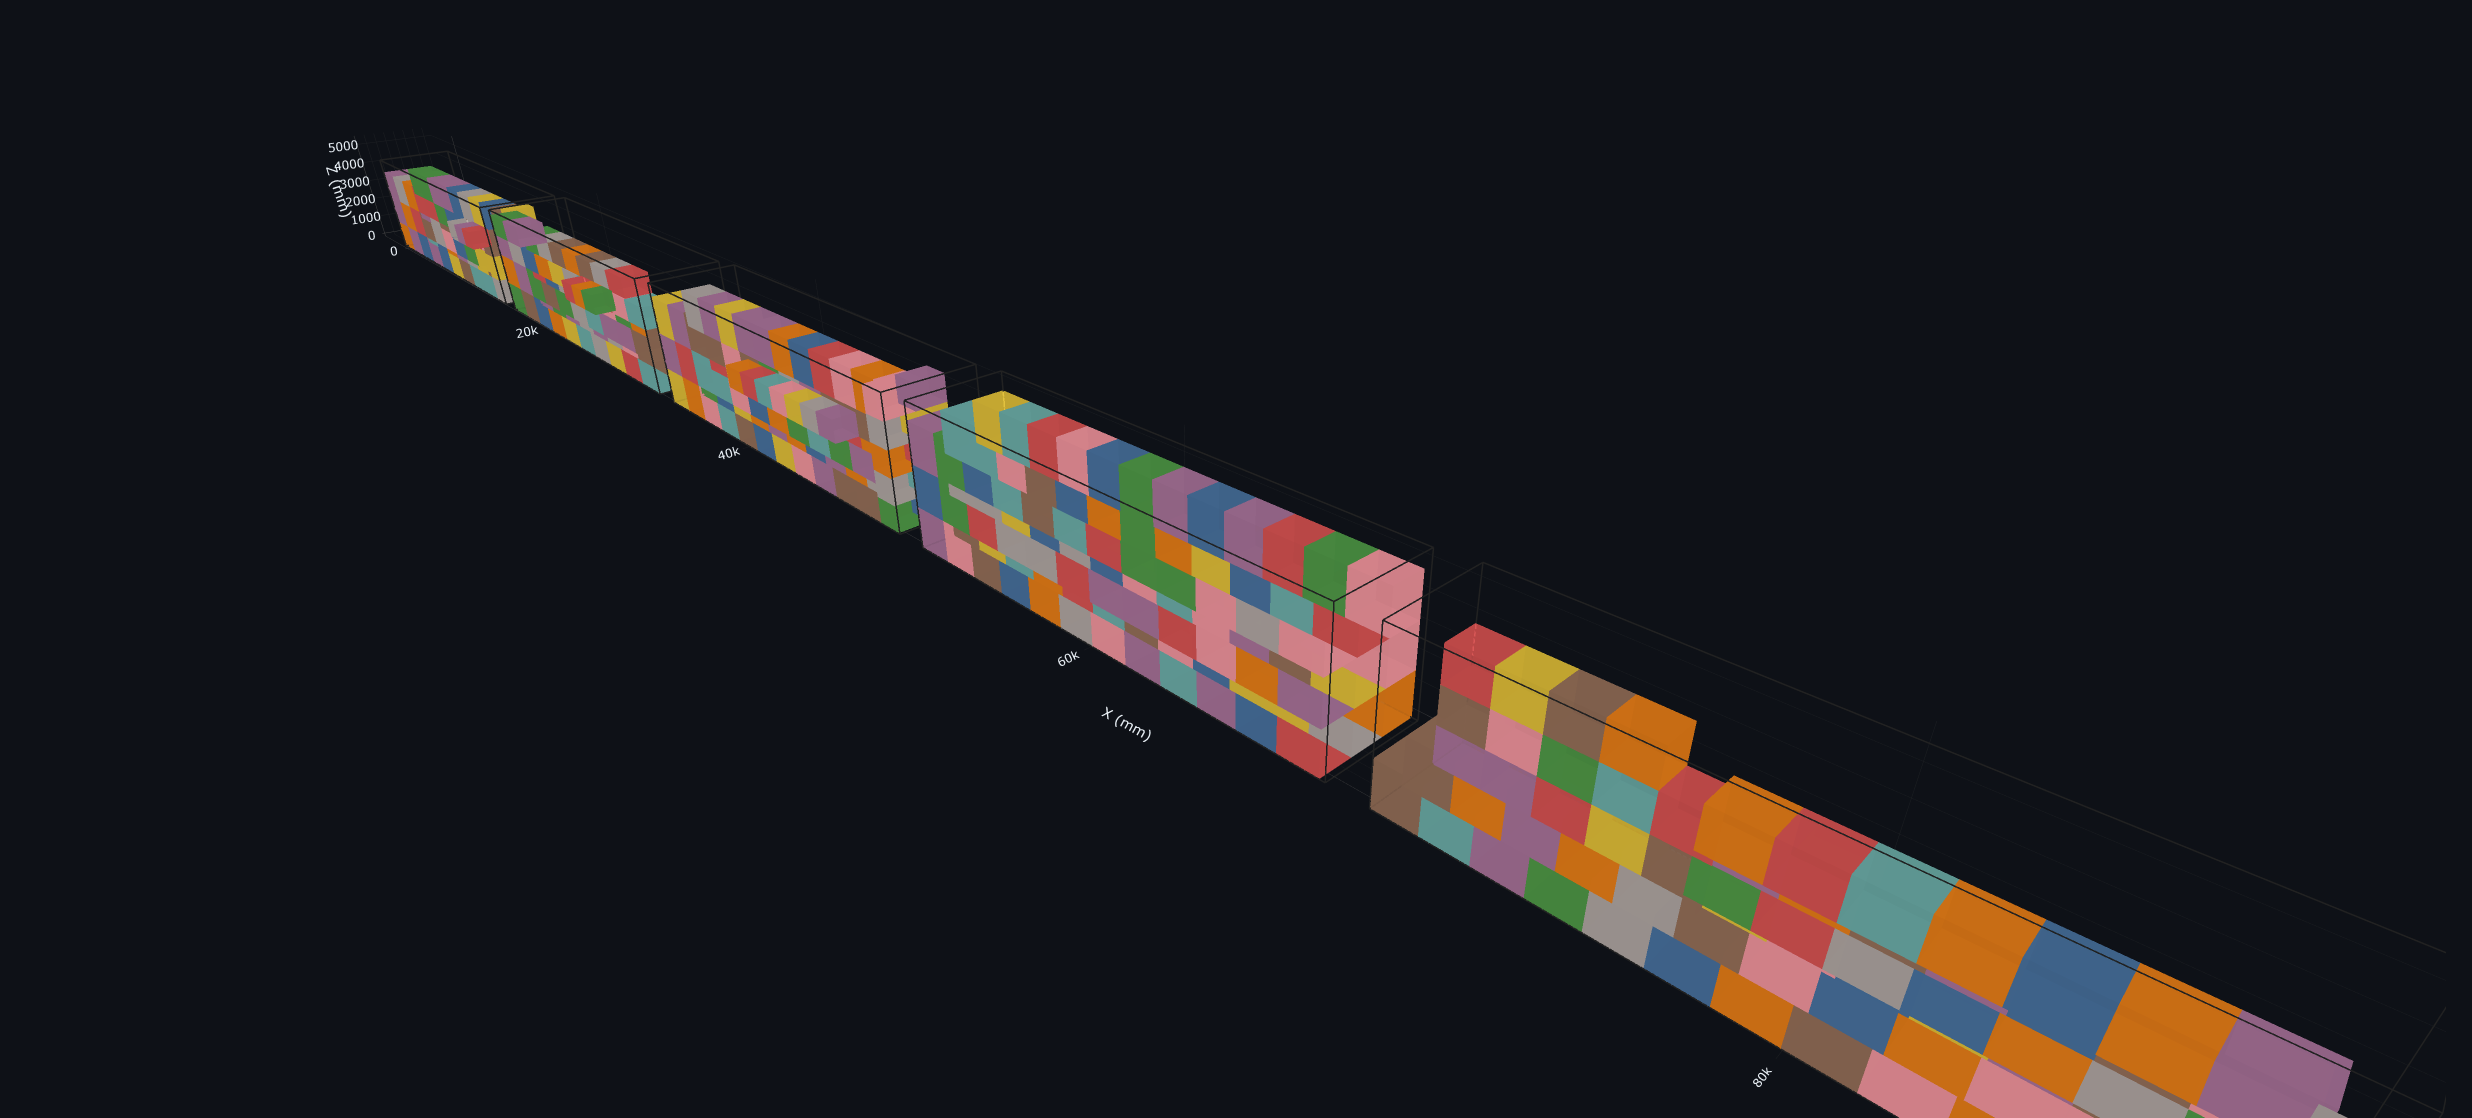
\includegraphics[width=\textwidth]{container-packing-500-items.png}
  \caption{Ví dụ nghiệm 3D đa-container với 500 kiện. Các container được nối tiếp trên
  trục X để dễ quan sát; khoảng cách giữa chúng chỉ phục vụ trực quan hóa.}
  \label{fig:packing-500}
\end{figure}

\section{Kiến trúc và luồng xử lý}

\begin{figure}[H]
\centering
\resizebox{\textwidth}{!}{%
\begin{tikzpicture}[
  node distance=8mm,
  stage/.style={rectangle, rounded corners, draw=brandblue, fill=softblue,
                minimum height=12mm, text width=24mm, align=center, font=\small},
  arrow/.style={-{Latex[length=2.5mm]}, thick, draw=brandblue}
]
  \node[stage] (data) {Dữ liệu kiện và kho};
  \node[stage, right=of data] (pre) {Chuẩn hóa và precheck};
  \node[stage, right=of pre] (subset) {Tìm subset container};
  \node[stage, right=of subset] (build) {Xây dựng phương án};
  \node[stage, right=of build] (repair) {Repair tùy chọn};
  \node[stage, right=of repair] (valid) {Kiểm định độc lập};
  \node[stage, right=of valid] (report) {Báo cáo và mô phỏng 3D};
  \draw[arrow] (data) -- (pre);
  \draw[arrow] (pre) -- (subset);
  \draw[arrow] (subset) -- (build);
  \draw[arrow] (build) -- (repair);
  \draw[arrow] (repair) -- (valid);
  \draw[arrow] (valid) -- (report);
\end{tikzpicture}%
}
\caption{Pipeline chuẩn từ dữ liệu gốc đến nghiệm đã kiểm định và mô phỏng.}
\end{figure}

\begin{enumerate}[leftmargin=1.7em]
  \item \textbf{Chuẩn hóa:} kiểm tra schema, đơn vị, ID và tương thích cơ bản.
  \item \textbf{Precheck:} tính cận sức chứa. Precheck đạt không đồng nghĩa đã chứng minh
  khả thi về hình học.
  \item \textbf{Construction:} chọn container, hướng đặt và tọa độ cho từng kiện.
  \item \textbf{Repair:} tùy chọn thử giảm container hoặc chi phí; không được làm mất
  incumbent đã hợp lệ.
  \item \textbf{Independent validation:} tính lại constraint từ dữ liệu gốc thay vì tin
  trực tiếp kết luận solver.
  \item \textbf{Reporting và 3D:} chỉ nghiệm complete và \code{VALID} mới có objective
  chính thức và scene hợp lệ.
\end{enumerate}

\section{Tiến trình bốn tuần}

\begin{longtable}{p{0.08\textwidth}p{0.40\textwidth}p{0.42\textwidth}}
\toprule
\textbf{Tuần} & \textbf{Thành quả chính} & \textbf{Ý nghĩa} \\
\midrule
\endfirsthead
\toprule
\textbf{Tuần} & \textbf{Thành quả chính} & \textbf{Ý nghĩa} \\
\midrule
\endhead
1 & Domain model, service thí nghiệm, validator và visualization 3D
  & Có luồng end-to-end từ input đến phương án hiển thị được. \\
2 & Support, xoay ngang, stackability, load-bearing và các heuristic/metaheuristic
  & Mở rộng constraint theo level mà không phá contract cũ. \\
3 & Inventory search, validated incumbent, bounded repair, EP/FFD/MES và benchmark
  & Tìm trong kho container và so sánh thuật toán công bằng hơn. \\
4 & Acceptance phân phối Level 3--5, profiling, recovery và cải thiện UI
  & Có evidence nhiều case, biết bottleneck và có luồng demo dễ sử dụng hơn. \\
\bottomrule
\end{longtable}

\section{Maturity Level 1--5}

\begin{longtable}{p{0.08\textwidth}p{0.27\textwidth}p{0.25\textwidth}p{0.30\textwidth}}
\toprule
\textbf{Level} & \textbf{Năng lực bổ sung} & \textbf{Trạng thái evidence} &
\textbf{Không được tuyên bố} \\
\midrule
\endfirsthead
\toprule
\textbf{Level} & \textbf{Năng lực bổ sung} & \textbf{Trạng thái evidence} &
\textbf{Không được tuyên bố} \\
\midrule
\endhead
1 & Hình học, non-overlap, payload, hướng cố định
  & Nghiên cứu đã nghiệm thu & Ổn định vật lý. \\
2 & Tiếp xúc sàn, exact support ratio, tâm đáy được đỡ
  & Nghiên cứu đã nghiệm thu & Ổn định động lực học đầy đủ. \\
3 & Xoay ngang \code{XYZ/YXZ}
  & Nghiên cứu đã nghiệm thu & Mọi phép xoay 3D tùy ý. \\
4 & Stackability, stack group và giới hạn layer
  & Nghiên cứu đã nghiệm thu & Độ bền vật liệu thực tế. \\
5 & Load-bearing và truyền tải trọng tĩnh đệ quy
  & Nghiên cứu đã nghiệm thu trên dữ liệu synthetic & Chứng nhận an toàn cơ học. \\
\bottomrule
\end{longtable}

Level 6--8 về nesting, cân bằng/trọng tâm và delivery/LIFO vẫn thuộc phạm vi nghiên cứu
tiếp theo, không được trình bày như thành phẩm hoàn thiện trong demo này.

\section{Thuật toán và objective chính thức}

Ba constructor chính đang được đánh giá:
\begin{description}[leftmargin=0pt,style=nextline]
  \item[Extreme Point Best Fit] Baseline thực dụng; đánh giá nhiều vị trí và chọn candidate
  phù hợp nhất theo ranking.
  \item[First Fit Decreasing (FFD)] Xếp kiện lớn trước và nhận vị trí khả thi đầu tiên;
  đơn giản, nhanh và deterministic.
  \item[Maximal Empty Spaces Best Fit (MES)] Theo dõi các vùng trống cực đại; có thể thắng
  ở một số nhóm case nhưng không thắng tuyệt đối.
\end{description}

Official objective là thứ tự từ điển:
\[
  \min\bigl(\text{used container count},\;\text{total container cost}\bigr).
\]
Trước khi so objective, candidate phải complete và independently \code{VALID}. Runtime và
utilization chỉ là chỉ số trade-off. Best Fit là baseline đối chiếu, không phải optimum đã
được chứng minh.

\section{Evidence đã có}

\subsection{Benchmark canonical Level 2}
\begin{itemize}[leftmargin=1.5em]
  \item 24 bài kiểm tra, 3 thuật toán, 2 repeat: 144 lượt.
  \item 144/144 lượt independently \code{VALID}; 72/72 nhóm deterministic.
  \item FFD so với Best Fit: 0 thắng / 24 hòa / 0 thua.
  \item MES so với Best Fit: 1 thắng / 22 hòa / 1 thua.
\end{itemize}

Kết quả cho thấy một hình ảnh hoặc một case không đủ để kết luận thuật toán tốt. Benchmark
phải ghép cặp các thuật toán trên cùng input, kho, constraint và deadline.

\subsection{Acceptance phân phối Level 3--5}

Mỗi Level có 84 bài và 756 lượt. Tổng cộng \good{2.268/2.268 lượt VALID}.

\begin{table}[H]
\centering
\begin{tabularx}{\textwidth}{lYY}
\toprule
\textbf{Level} & \textbf{FFD so với Best Fit} & \textbf{MES so với Best Fit} \\
\midrule
3 & 1 thắng / 59 hòa / 0 thua & 18 thắng / 38 hòa / 4 thua \\
4 & 1 thắng / 57 hòa / 2 thua & 32 thắng / 28 hòa / 0 thua \\
5 & 2 thắng / 57 hòa / 1 thua & 32 thắng / 28 hòa / 0 thua \\
\bottomrule
\end{tabularx}
\caption{So sánh ghép cặp trên nhóm random. Stress và prefix được báo riêng.}
\end{table}

Không so container count thô giữa các Level để xếp hạng vì mỗi Level có tập constraint
khác nhau. Chênh lệch giữa Level chỉ phản ánh chi phí của ràng buộc bổ sung.

\section{Profiling và bottleneck}

\begin{table}[H]
\centering
\begin{tabular}{lrrr}
\toprule
\textbf{Nhóm thời gian} & \textbf{Level 3} & \textbf{Level 4} & \textbf{Level 5} \\
\midrule
Construction / wall time & 59,6\% & 70,9\% & 71,6\% \\
Support/contact/constraint self-time & 18,7\% & 54,6\% & 58,7\% \\
Reporting / wall time & 15,5\% & 11,0\% & 10,1\% \\
\bottomrule
\end{tabular}
\caption{Tỷ trọng thời gian từ profiling chẩn đoán.}
\end{table}

Construction là phase chi phối. Ở Level 4--5, kiểm tra contact/support và constraint liên
quan chiếm hơn một nửa profiled solver self-time. Vì vậy hướng ưu tiên là A/B cache hoặc
contact/support index dùng chung; tối ưu reporting chưa phải ưu tiên đầu tiên.

\section{Kịch bản demo local 15 phút}

\subsection{Checklist trước demo}
\begin{enumerate}[leftmargin=1.7em]
  \item Kiểm tra Python trong virtual environment.
  \item Chạy smoke test Streamlit.
  \item Khởi động ứng dụng trước giờ trình bày.
  \item Mở sẵn báo cáo này, ảnh 500 kiện và evidence Level 2 làm fallback.
  \item Không chạy benchmark 144/756 lượt trong buổi demo.
\end{enumerate}

\begin{lstlisting}
Set-Location D:\IT\Project\gsm\3DBinPacking
.\.venv\Scripts\python.exe --version
.\.venv\Scripts\python.exe -m pytest -q tests\test_streamlit_app.py
.\.venv\Scripts\python.exe .\scripts\run_web_app.py
\end{lstlisting}

\subsection{Thiết lập demo Level 2}
\begin{table}[H]
\centering
\begin{tabularx}{\textwidth}{p{0.43\textwidth}Y}
\toprule
\textbf{Mục} & \textbf{Giá trị} \\
\midrule
Nguồn dữ liệu & 1.000 kiện / 500 container / 10 loại \\
Thuật toán & Extreme Point -- Best Fit Decreasing \\
Số kiện & 100 \\
Tìm container trong toàn kho & Bật \\
Số container bắt đầu / tự tăng & 1 / Bật \\
Số container tối đa & 10 \\
Thời gian tối đa & 60 giây \\
Repair sau construction & Tắt \\
\bottomrule
\end{tabularx}
\end{table}

\subsection{Timeline và câu thoại gợi ý}
\begin{longtable}{p{0.12\textwidth}p{0.26\textwidth}p{0.52\textwidth}}
\toprule
\textbf{Thời gian} & \textbf{Thao tác} & \textbf{Thông điệp} \\
\midrule
\endfirsthead
\toprule
\textbf{Thời gian} & \textbf{Thao tác} & \textbf{Thông điệp} \\
\midrule
\endhead
0--2 phút & Mở bài toán và ảnh 3D
& Hệ thống chọn container, tọa độ và hướng đặt; ưu tiên ít container rồi chi phí. \\
2--4 phút & Chỉ sơ đồ pipeline
& Solver không tự chấm; nghiệm phải qua validator độc lập từ input gốc. \\
4--10 phút & Chạy Level 2 với cấu hình trên
& 500 container là kho khả dụng, không phải số bắt buộc dùng; hệ thống mở thêm khi cần. \\
10--12 phút & Đọc kết quả và xoay mô hình 3D
& \code{VALID} là đã qua validator. Khoảng trống có thể do payload, hình học hoặc support. \\
12--14 phút & Mở evidence benchmark đã lưu
& Một case chỉ chứng minh service chạy; đánh giá thuật toán cần nhiều case ghép cặp công bằng. \\
14--15 phút & Kết luận và roadmap
& Core đã có evidence; bottleneck kế tiếp là contact/support trong construction. \\
\bottomrule
\end{longtable}

\section{Phương án dự phòng}

\begin{longtable}{p{0.30\textwidth}p{0.60\textwidth}}
\toprule
\textbf{Sự cố} & \textbf{Cách xử lý trong buổi demo} \\
\midrule
\endfirsthead
\toprule
\textbf{Sự cố} & \textbf{Cách xử lý trong buổi demo} \\
\midrule
\endhead
Streamlit chưa mở & Chạy lại \code{scripts/run_web_app.py}; tiếp tục trình bày tài liệu trong lúc chờ. \\
Run 100 kiện lâu bất thường & Đổi xuống 20 kiện; không tăng timeout vô hạn. \\
Không có scene & Đọc reason code; dùng Hình~\ref{fig:packing-500} và evidence đã lưu. \\
Mạng bị chặn & Demo local không phụ thuộc GitHub hoặc Internet. \\
Lịch sử benchmark không xuất hiện & Mở report đã commit, không chạy lại corpus dài. \\
\bottomrule
\end{longtable}

\section{Câu hỏi thường gặp}

\textbf{Đây đã là giải pháp tối ưu chưa?}

Chưa. Heuristic tạo nghiệm hợp lệ và thực dụng nhưng không chứng minh tối ưu. Best Fit là
baseline; aggregate lower bound chỉ là cận sức chứa sơ bộ.

\textbf{Tại sao container còn khoảng trống?}

Không gian trống có thể do payload đã đầy, hình học không tương thích, yêu cầu support/chồng
xếp hoặc heuristic chưa tìm được cách gom tốt hơn.

\textbf{Benchmark có phải một thuật toán chuẩn không?}

Không. Benchmark là protocol gồm dataset, danh sách case, thuật toán, seed, deadline, repeat
và cách tổng hợp. Các thuật toán chạy trên cùng case rồi mới so thắng/hòa/thua.

\textbf{Có chạy được 10.000--100.000 kiện không?}

Pipeline dữ liệu có profile lớn, nhưng solver quy mô đó chưa qua acceptance runtime/memory.
Demo và evidence chính hiện sử dụng nguồn 1.000 kiện / 500 container.

\textbf{Kết quả có dùng trực tiếp để xếp hàng thật không?}

Chỉ sau khi thay dữ liệu synthetic bằng dữ liệu thực có provenance, hiệu chỉnh constraint
vật lý và hoàn thành acceptance/SLA production.

\section{Thuật ngữ}

\begin{longtable}{p{0.24\textwidth}p{0.66\textwidth}}
\toprule
\textbf{Thuật ngữ} & \textbf{Giải thích ngắn} \\
\midrule
\endfirsthead
\toprule
\textbf{Thuật ngữ} & \textbf{Giải thích ngắn} \\
\midrule
\endhead
Heuristic & Quy tắc tìm nghiệm nhanh, không bảo đảm nghiệm tối ưu. \\
Benchmark & Bộ bài kiểm tra và protocol cố định để so sánh công bằng. \\
Case & Một input cụ thể: tập kiện, kho, constraint và giới hạn chạy. \\
Execution & Một lần một thuật toán chạy trên một case. \\
Validator & Thành phần độc lập tính lại constraint từ input và solution. \\
Lower bound & Cận dưới sơ bộ; không thể dùng ít hơn nhưng chưa chắc đạt được. \\
Inventory search & Tìm tổ hợp physical container phù hợp trong toàn bộ kho. \\
Incumbent & Nghiệm hợp lệ tốt nhất đang được giữ trong quá trình tìm kiếm. \\
Repair & Bước tùy chọn thử cải thiện incumbent sau construction. \\
Profiling & Đo thời gian từng phase/hàm để xác định bottleneck. \\
Deterministic & Cùng input/config/seed cho cùng objective và placement signature. \\
WIP & Work in progress: sản phẩm đang hoàn thiện, chưa phải bản production. \\
\bottomrule
\end{longtable}

\section{Tài liệu đối chiếu}

\begin{itemize}[leftmargin=1.5em]
  \item Mục lục tài liệu: \code{docs/index.md}.
  \item Contract Level 1--5: \code{docs/levels/level_01.md} đến
  \code{docs/levels/level_05.md}.
  \item Hướng dẫn Streamlit: \code{docs/guides/running_web_app.md}.
  \item Evidence Level 2:
  \code{docs/reports/manual/level_02_canonical_benchmark_20260813.md}.
  \item Acceptance và profiling Level 3--5:
  \code{docs/reports/manual/level_03_05_distribution_20260814/cross_level_distribution_report.md}.
\end{itemize}

\section*{Giới hạn của báo cáo}
\addcontentsline{toc}{section}{Giới hạn của báo cáo}

Các số liệu trong báo cáo phản ánh contract phần mềm và corpus nghiên cứu tại thời điểm
15/08/2026. Dữ liệu phần lớn là synthetic/research. Báo cáo không chứng nhận an toàn cơ
học, không cam kết SLA production và không tuyên bố các heuristic đạt optimum toàn cục.

\end{document}
